% =====================================================================
%  §8. Правдоподобие, информационный критерий, анализ остатков
%
%  ЖАНР (STYLE.md): учебная литература. Ни путей, ни имён программ, ни
%  номеров гипотез. Прослеживаемость — ключи \srckey{8.x} и приложение.
%
%  Содержательная основа: BRIEF_FOR_D_teaching_ladder.md §9; SYNTHESIS.md §6.
% =====================================================================
\section{Правдоподобие, информационный критерий, анализ остатков}
\label{sec:likelihood}
\markboth{§\thesection. Правдоподобие и остатки}{}

Информационный критерий уже дважды использовался в курсе (§6~--- лестница моделей, §7~---
качество областей притяжения) как готовый инструмент со ссылкой «объяснение~--- в §8». Здесь
даётся обоснование: откуда вообще берётся штраф $2k$ и почему минимизация суммы квадратов~---
не техническая условность, а частный случай гораздо более общего принципа. Вторая половина
параграфа~--- то, что происходит \emph{после} подгонки: анализ остатков, обязательная, а не
факультативная часть работы, потому что хороший $\chi^2$ сам по себе ничего не говорит о том,
не остался ли в данных сигнал, который модель не объяснила.

\begin{tcolorbox}[enhanced,colback=cPanel,colframe=cGrid,boxrule=0.8pt,arc=2pt,
                  title={\bfseries\color{cAccent} Пререквизиты},coltitle=cAccent,
                  attach boxed title to top left={xshift=6pt,yshift=-2pt},
                  boxed title style={colback=cPanel,boxrule=0pt,arc=0pt},top=10pt]
\textbf{Нужно знать:} §6 (лестница моделей, качественная шкала $\dAIC$); §7 (целевая функция,
веса); нормальное распределение и его функция плотности.\\[0.3em]
\textbf{Знать НЕ нужно:} байесовский вывод информационных критериев~--- здесь используется
классический (частотный) вывод AIC Акаике, в его наиболее прикладной форме.
\end{tcolorbox}

% ---------------------------------------------------------------------
\subsection{От суммы квадратов к правдоподобию}
\label{subsec:likelihood}

\begin{strict}[: минимизация $\chi^2$ есть максимизация правдоподобия]
Пусть измерения $y_i$ отличаются от истинных значений модели $f(\mathbf{p};x_i)$ независимым
гауссовым шумом с известной дисперсией~$\sigma_i^2$. Плотность вероятности всего набора
измерений при данных параметрах~$\mathbf{p}$~--- \term{функция правдоподобия}:
\[
  L(\mathbf{p})=\prod_i\frac{1}{\sqrt{2\pi}\sigma_i}
  \exp\!\left[-\frac{(y_i-f(\mathbf{p};x_i))^2}{2\sigma_i^2}\right] .
\]
Её логарифм~--- сумма, а не произведение:
\[
  \ln L(\mathbf{p})=-\frac12\sum_i\frac{(y_i-f(\mathbf{p};x_i))^2}{\sigma_i^2}
  -\sum_i\ln(\sqrt{2\pi}\sigma_i)
  =-\tfrac12\chi^2(\mathbf{p})+\text{const} .
\]
Второе слагаемое от~$\mathbf{p}$ не зависит. Значит, тот параметр~$\mathbf{p}$, который
\emph{максимизирует} правдоподобие,~--- тот же самый, что \emph{минимизирует}~$\chi^2$ из
формулы~\eqref{eq:objective}. Взвешенный МНК всех предыдущих параграфов~--- не отдельный метод,
а максимизация правдоподобия в частном случае гауссова шума с весами $w_i=1/\sigma_i^2$.
\end{strict}

\begin{intuition}
Это не просто переобозначение. Как только подгонка признана максимизацией правдоподобия, к ней
становится применим весь аппарат статистического вывода, разработанный именно для правдоподобия,~---
в частности, сравнение моделей разной сложности, к которому курс и переходит.
\end{intuition}

% ---------------------------------------------------------------------
\subsection{Информационный критерий: плата за параметр}
\label{subsec:aic}

\begin{intuition}
Добавление любого нового параметра не может ухудшить максимум правдоподобия на тех же данных, на
которых модель обучена,~--- в худшем случае оптимизатор просто им не воспользуется. Сравнение
моделей по одному лишь $\ln L$ (или $\chi^2$) поэтому всегда предпочтёт более сложную модель, даже
если новый параметр не отражает никакой реальной структуры данных, а просто <<подстраивается>> под
шум. Нужна поправка, штрафующая за каждый дополнительный параметр,~--- она и называется
\term{информационным критерием Акаике}:
\begin{equation}
  \AIC=-2\ln L+2k,
  \label{eq:aic}
\end{equation}
где $k$~--- число свободных параметров модели. Из двух моделей предпочтительна та, у которой
$\AIC$ \emph{меньше}: она либо объясняет данные не хуже при меньшей сложности, либо оправдывает
дополнительную сложность реальным выигрышем в правдоподобии, превышающим штраф $2k$.
\end{intuition}

\noindent
Практическая шкала, уже использованная без обоснования в §6--§7 (общепринятая в статистической
литературе, число $10$~--- условный, но широко принятый порог):

\begin{center}
\footnotesize
\setlength{\tabcolsep}{8pt}
\begin{tabular}{@{}lp{0.62\linewidth}@{}}
\toprule
$|\dAIC|$ & \textbf{Что это означает} \\
\midrule
$\lesssim2$    & модели практически неразличимы данными \\
$2$--$10$      & умеренное свидетельство в пользу модели с меньшим $\AIC$ \\
$\gtrsim10$    & уверенное предпочтение \\
$\gtrsim$ сотни--тысячи & прежняя модель категорически не годится (пример~--- пин к физическому
диаметру, §6) \\
\bottomrule
\end{tabular}
\end{center}

\begin{warning}[: условие, без которого сравнение бессмысленно]
Формула~\eqref{eq:aic} сравнивает модели \emph{на одних и тех же данных}. Если у сравниваемых
вариантов разный набор точек, разные веса или разный способ построения предсказания, разность
$\AIC$ перестаёт что-либо означать~--- штраф $2k$ откалиброван на предположении, что единственное
отличие моделей~--- число параметров, а не подмена задачи. Вся лестница §6 построена так, что все
её ступени используют один и тот же набор точек и одни и те же веса именно по этой причине.
\end{warning}

% ---------------------------------------------------------------------
\subsection{Анализ остатков: обязательная проверка, а не украшение}
\label{subsec:residuals}

Хороший $\AIC$ говорит: «эта модель лучше той». Он не говорит: «эта модель исчерпала данные».
Ответ на второй вопрос даёт \term{остаток}~--- разность между измерением и предсказанием
наилучшей модели,~--- и то, насколько он похож на чистый шум.

\paragraph{Нормальность.} Если модель верна, а шум прибора гауссов, остаток должен быть похож на
выборку из нормального распределения. Стандартные проверки~--- критерии Шапиро--Уилка и
Жарка--Бера (числовые статистики) и \term{график квантиль-квантиль} (Q--Q): по оси абсцисс~---
квантили, которые дало бы точное нормальное распределение, по оси ординат~--- квантили реального
остатка. Если распределения совпадают, точки ложатся на прямую; систематическое отклонение от
прямой (особенно на хвостах) выдаёт структуру, которой в чистом шуме быть не должно.

\paragraph{Автокорреляция.} \term{Статистика Дарбина--Уотсона} измеряет корреляцию остатка с самим
собой, сдвинутым на один отсчёт: значение вблизи~$2$ означает отсутствие автокорреляции (белый
шум), значения, заметно меньшие двух, означают, что соседние точки остатка похожи друг на
друга~--- то есть в данных осталась \emph{структура}, которую модель не объяснила, а не случайный
разброс.

\begin{example}[: две крайности одного проекта]\srckey{8.1}
На плотной решётке после включения всех поправок опорной модели (§6) статистика
Дарбина--Уотсона остатка по амплитуде составляет $\approx0{,}32$~--- далеко от идеала~$2$: остаток
всё ещё заметно структурен, модель не полна. На разреженном образце та же статистика после той же
модели даёт $\approx1{,}76$~--- почти белый шум: там модель практически исчерпала данные. Одна и
та же модель, применённая к двум образцам, оставляет принципиально разное количество необъяснённой
структуры~--- сам факт этого различия является диагностикой не хуже, чем абсолютное значение.
\end{example}

% ---------------------------------------------------------------------
\begin{figure}[t]
  \centering
  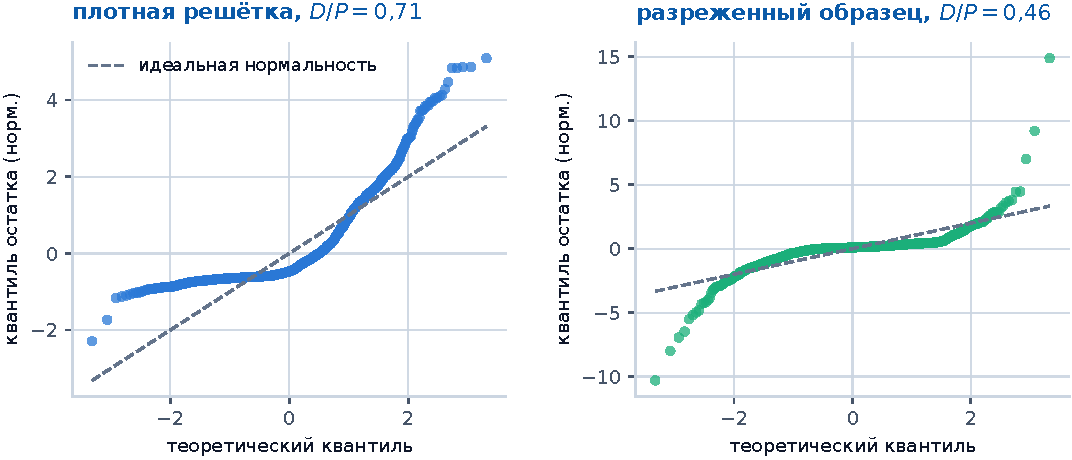
\includegraphics[width=\linewidth]{figures/fig08_qq.pdf}
  \caption{График квантиль-квантиль остатка амплитуды (плотная решётка против разреженного
  образца, модель без явного просачивания~--- тот же срез, на котором была впервые замечена
  структура остатка, обсуждаемая ниже). Прямая линия отвечала бы точной нормальности;
  систематическое искривление на краях, заметно более выраженное для плотной решётки, выдаёт
  негауссовость остатка.}
  \label{fig:qq}
\end{figure}

\paragraph{Карты остатков.} Если остаток зависит и от угла, и от частоты, полезно смотреть не на
одномерные срезы, а на двумерную карту угол\,$\times$\,частота: локализованное <<пятно>> отклонения
подсказывает физический механизм гораздо точнее, чем усреднённая по всем точкам статистика.

\begin{example}[: так был найден дефицит тени]\srckey{8.2}
Именно карта остатков угол\,$\times$\,частота, построенная для модели без явного просачивания,
впервые локализовала систематическую недооценку сигнала в глубокой тени~--- порядка $3$--$4$~дБ, и
только на плотном образце, а не разреженном. Это наблюдение и стало отправной точкой для введения
явного просачивания в §1 и §6: карта остатков не просто зафиксировала, что модель <<не идеальна>>,
а указала, \emph{где именно} и \emph{насколько}, что резко сузило круг гипотез.
\end{example}

\begin{figure}[t]
  \centering
  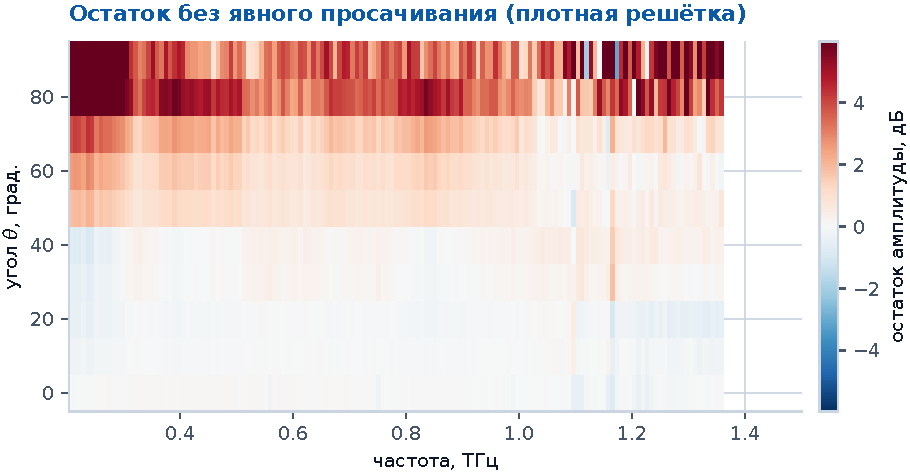
\includegraphics[width=\linewidth]{figures/fig08_residual_map.pdf}
  \caption{Карта остатка амплитуды (угол против частоты) для плотной решётки, модель без явного
  просачивания. Систематическое усиление отклонения к большим углам~--- то самое наблюдение,
  которое привело к введению просачивания в опорную модель курса (§1, §6).}
  \label{fig:residual-map}
\end{figure}

\paragraph{Разложение остатка по осям.} После того как явное просачивание уже включено в модель
(§6), остаток на плотном образце всё ещё содержит два опознаваемых компонента: локализованный
<<горячий>> пик на низкой частоте (около $0{,}21$--$0{,}22$~ТГц, амплитуда порядка $1{,}7$--$1{,}8$~дБ)
и гладкий дисперсионный наклон около $-0{,}62$~дБ на терагерц по всей полосе. Ни то, ни другое
пока не отнесено к конкретному физическому механизму с уверенностью~--- это открытый остаток,
честно предъявленный, а не спрятанный.\srckey{8.3}

\paragraph{Проверка на отложенных данных (held-out).} Самая строгая проверка~--- не то, насколько
хорошо модель описывает те же данные, на которых обучена, а то, переносится ли параметр,
измеренный на одной части данных, на другую. Просачивание, оценённое по яркой части развёртки
(там, где сигнал велик и шум относительно мал), можно проверить, подставив его в предсказание для
тени~--- части данных, не участвовавшей в этой оценке.

\begin{example}[: хороший фит — не то же самое, что предсказательная сила]\srckey{8.4}
Параметр амплитуды просачивания, определённый по ярким углам, даёт среднеквадратичную ошибку
$0{,}50$~дБ на самих ярких углах, но $3{,}75$~дБ при попытке предсказать глубокую тень~---
почти в восемь раз хуже. Мораль: способность модели хорошо описать те данные, по которым
оценивался параметр,~--- необходимое, но не достаточное условие того, что параметр физически верно
характеризует весь диапазон измерения.
\end{example}

% ---------------------------------------------------------------------
\subsection{Различение, ради которого всё это делается}
\label{subsec:distinction}

\begin{tcolorbox}[enhanced,colback=cS1!7,colframe=cS1,boxrule=0pt,leftrule=3pt,arc=1pt]
\textbf{«Модель лучше описывает данные» и «параметр модели измерен» — разные утверждения.} Курс
уже трижды сталкивался с этим различением по частям: показатель рассеяния~$\gamma$ (§3)~---
эффект реален, конкретное значение плывёт в разы в зависимости от соседних членов модели;
перекрёстный член (§6)~--- улучшает $\AIC$ на одном образце, не проходит проверку однородности
между образцами; амплитуда просачивания (только что, §\ref{subsec:residuals})~--- хорошо описывает
те данные, по которым получена, но не экстраполируется. §9 соберёт это различение в общий
формальный аппарат~--- информацию Фишера и профильное правдоподобие,~--- которым можно проверять
его заранее, не дожидаясь held-out теста по факту.
\end{tcolorbox}

% ---------------------------------------------------------------------
\subsection{Типичные ошибки этого параграфа}

\begin{enumerate}[leftmargin=1.6em,itemsep=0.25em]
  \item Сравнивать модели по $\AIC$, посчитанному на разных наборах точек или с разными весами.
        Штраф $2k$ откалиброван на предположении, что данные и способ их взвешивания общие
        (§\ref{subsec:aic}).
  \item Считать хороший $\chi^2$ или $\AIC$ достаточным основанием не смотреть на остатки. Модель
        может быть <<лучшей из предложенных>> и одновременно далёкой от исчерпания данных
        (пример со статистикой Дарбина--Уотсона, §\ref{subsec:residuals}).
  \item Усреднять остаток по одной из осей (только по углу или только по частоте) прежде, чем
        проверить двумерную карту. Локализованный дефект легко потерять при усреднении.
  \item Считать, что параметр, хорошо описывающий обучающую часть данных, автоматически годится
        для экстраполяции. Held-out проверка~--- отдельный и более строгий тест
        (§\ref{subsec:residuals}).
  \item Путать «эффект статистически значим» с «параметр физически измерен»~--- это ровно то
        различение, ради которого написан весь параграф (§\ref{subsec:distinction}).
\end{enumerate}

\clearpage
